% !TEX encoding = UTF-8 Unicode
\documentclass[a4paper]{article}

\usepackage[utf8]{inputenc}
\usepackage{erk}
\usepackage{amsmath}
\usepackage{times}
\usepackage{graphicx}
\usepackage{hyperref}
\usepackage[top=22.5mm, bottom=22.5mm, left=22.5mm, right=22.5mm]{geometry}

\usepackage[slovene,english]{babel}

% local definitions
\def\footnotemark{}%  to avoid footnote on cover page

\begin{document}
%make title
\title{Deformacija vhoda v funkcijo atan2 in potek napake v odvistnosti od deformacije}

\author{Mitja Alič} % use ^1, ^2 for author(s) from different institutions

\affiliation{Fakulteta za elektrotehniko, Univerza v Ljubljani, Tržaška cesta 25, 1000 Ljubljana}

\email{E-pošta: mitja1357@gmail.com}

\maketitle


\begin{abstract}{Distortion of the input to the atan2 function and the course of error due to distortion}
Distortion of sine and cosine used for angle identification, causes error. By different literature, error is presented by basic harmonic only. My project is to present error with higher harmonics inclouded, due to non-equalities of amplitudes of basic sine and cosine, offsets and non-ortogonality.
%Popačenje signalov sinus in kosinus, katera se uporablja določitev kota, nam ustvari napako. Napaka se različno obnaša glede na deformacijo. Literatura navaja osnovne harmonike napake. Raziskal sem kako se obnašajo višji harmoniki napake ob deformaciji sinus in kosinus signala s popačenimi amplitudami, neortogonalnimi fazami ter enosmernimi komponentami.
\end{abstract}


\selectlanguage{slovene}

\section{Uvod}

Dandanes je potreba po kakovostni regulaciji elektromotorskih pogonov neizogibna. Za kakovostno nadzorovanje rotirajočega pogona, se v povratnih zankah uporablja senzorje zasuka. Zasuk se meri na različne principe, inkrementalni dajalnik, resolver, enkoder... Resolver in enkoder, na podlagi zajetih signalov, v obliki sinusa in kosinusa, določi kot. Za izračun kota, se uporablja funkcija atan2.

Senzorji niso idealni in napaka je neizogibna. Primer napake je nepopolna oblika, zajetih signalov sinus in cosinus. V tem delu, bom predstavil, kako se izraža napaka izmerjenega kota, pri deformiranih vhodnih signalih sinusa in kosinusa.

Različne literature \cite{RLS1}, \cite{RLS2}, \cite{RLS3} opisujejo, kako deformacija vhodnih signalov vpliva na napako. Napako so izrazili le z najočitnejšimi harmoniki. V napaki nastopajo tudi višji harmoniki, katre se lahko predstavi, kot napaka v obliki  neskončne vrste (\ref{equ:potek_napake}).
\begin{equation}
\label{equ:potek_napake}
\varepsilon(x) = C_0(x) + \sum_{n=1}^{\infty} C_n(x) \sin(n \Theta+ \varphi_n(x))
\end{equation}
Parameter x predstavlja, neodvisno spremenljivko, katera popači vhodna signala sinus in kosinus. $C_0$ predstavlja enosmerno komponento napake, $C_n$ amplitudo posameznega člena vrste ter $\varphi_n$ fazni zamik harmonika napake. Vsi členi so odvisni od x.

Osnovna vhodna signala sinus in kosinus sta:
\begin{eqnarray}
\label{equ:def_sin}
&Sin = B_{0} + B_1 \sin(\theta + \varphi_{s})\\
\label{equ:def_cos}
&Cos = A_{0} + A_1 \cos(\theta + \varphi_{c})
\end{eqnarray}
Idealno so v (\ref{equ:def_sin}) in (\ref{equ:def_cos}), $B_0$, $A_0$, $\varphi_{s}$ in $\varphi_{c}$, enaki 0, $B_1$ in $A_1$ sta enaki. V nadaljevanju bom opisal, kako se izrazi napaka pri neenakosti $B_1$ in $A_1$. Opisal bom tudi odvistnost napake, pri neničelnosti enosmernih komponent ter če sta $B_0$, $A_0$ enaka. Opisal bom tudi, kako se izrazi napaka, če se vhodnima signaloma prišteje, signal v obliki sinusa ali kosinusa. Tako popačenje povzroči različni amplitudi in različna fazna kota v odvisntnosti od ene spremenljivke. 
\begin{eqnarray}
\label{equ:def_eks_sin}
&Sin = \sin(\theta)+\Delta_c \cos(\theta)+\Delta_s \sin(\theta)\\
\label{equ:def_ek_cos}
&Cos =\cos(\theta)+\Delta_c \cos(\theta)+\Delta_s \sin(\theta)
\end{eqnarray}

\section{Metode}

Definicija merjenega kota $\varphi$ in  napake $\varepsilon$ je:

\begin{eqnarray}
\label{equ:def_kot}
&\varphi = \mathrm{atan2d}(Sin,Cos)\\
\label{equ:def_err}
&\varepsilon =\varphi - \mathrm{atan2d}(\sin(\theta),\cos(\theta))
\end{eqnarray}
pri čemer $\theta$ predstavlja referenco.

Funkcija atan2d() je definirana funkcija v programskem okolju MATLAB, katera izračuna vrednost atan v štirih kvadrantih in izhod je v stopinjah\cite{atan}. Vsi rezultati so predstavljeni v stopinjah.

Določanja napake sem se lotil na naslednji način. Izbran parameter, katerega sem upošteval pri napaki, sem limitiral v neskončnost. Pri limitiranju parametra v neskončnost, se napaka izrazi v obliki npr:
\begin{equation}
\label{equ:def_err_inf}
\varepsilon=
\begin{cases}
90^\circ-\theta, & \theta \in \{0^\circ,180^\circ\}\\
270^\circ-\theta, & \theta \in \{180^\circ,360^\circ\}
\end{cases}
\end{equation}
Napako se da razviti v Fourierovo vrsto \cite{fourier} in s tem ugotoviti, k čemu strmi ob večanju parametra ter katere harmonike je pomembno opazovati. Sledi iskanje analitične funkcije, ki opisuje potek amplitude harmonika ter faznega zasuka posameznega harmonika, ob spremembi parametra. Ugotovil sem, da so višji harmoniki podobni osnovnemu harmoniku napake, le potencirani. Napaka se izrazi kot potenčna vrsta.

\subsection{Določanje napake ob različnih amplitudah}

Z uporabo sistema per unit in bazo $A_1$ se sistem poenostavi v sistem z eno spremenljivko. Razmerje amplitud definira koeficient k. Sprememba obeh amplitud za določen faktor, nebo ustvarila dodatne napake.
	\begin{eqnarray}
	\label{equ:def_sin_ama}
	&Sin = k \sin(\theta)\\
	\label{equ:def_cos_amp}
	&Cos =\cos(\theta)
	\end{eqnarray}
Ko gre k proti neskončnosti, se pojavi napaka (Slika \ref{fig:lim_amp})
\begin{equation}
\label{equ:amp_lim}
\lim_{k \rightarrow \infty} \mathrm{atan2}(k \sin{\theta},\cos{\theta})-\mathrm{atan2}(\sin{\theta},\cos{\theta})
\end{equation}
\begin{figure}[!htb]
	\begin{center}
		\includegraphics[width=\linewidth]{./Slike/lim_amp.eps}
		\caption{Napaka $\varepsilon$ ob limiti k} \label{fig:lim_amp}
	\end{center}
\end{figure}

predstavljena s Fourierovo vrsto
\begin{equation}
\label{equ:lim_amp_vrsta}
\varepsilon = \frac{180}{\pi}\sum_{n=1}^{\infty}\frac{1}{n} \sin 2 n \theta.
\end{equation}
Največni vpliv ima drugi harmonik. Potek drugega harmonika je predstavljen na sliki \ref{fig:amp} kot $C_1$, saj nastopajo le sodi harmoniki.
\begin{figure}[!htb]
	\begin{center}
		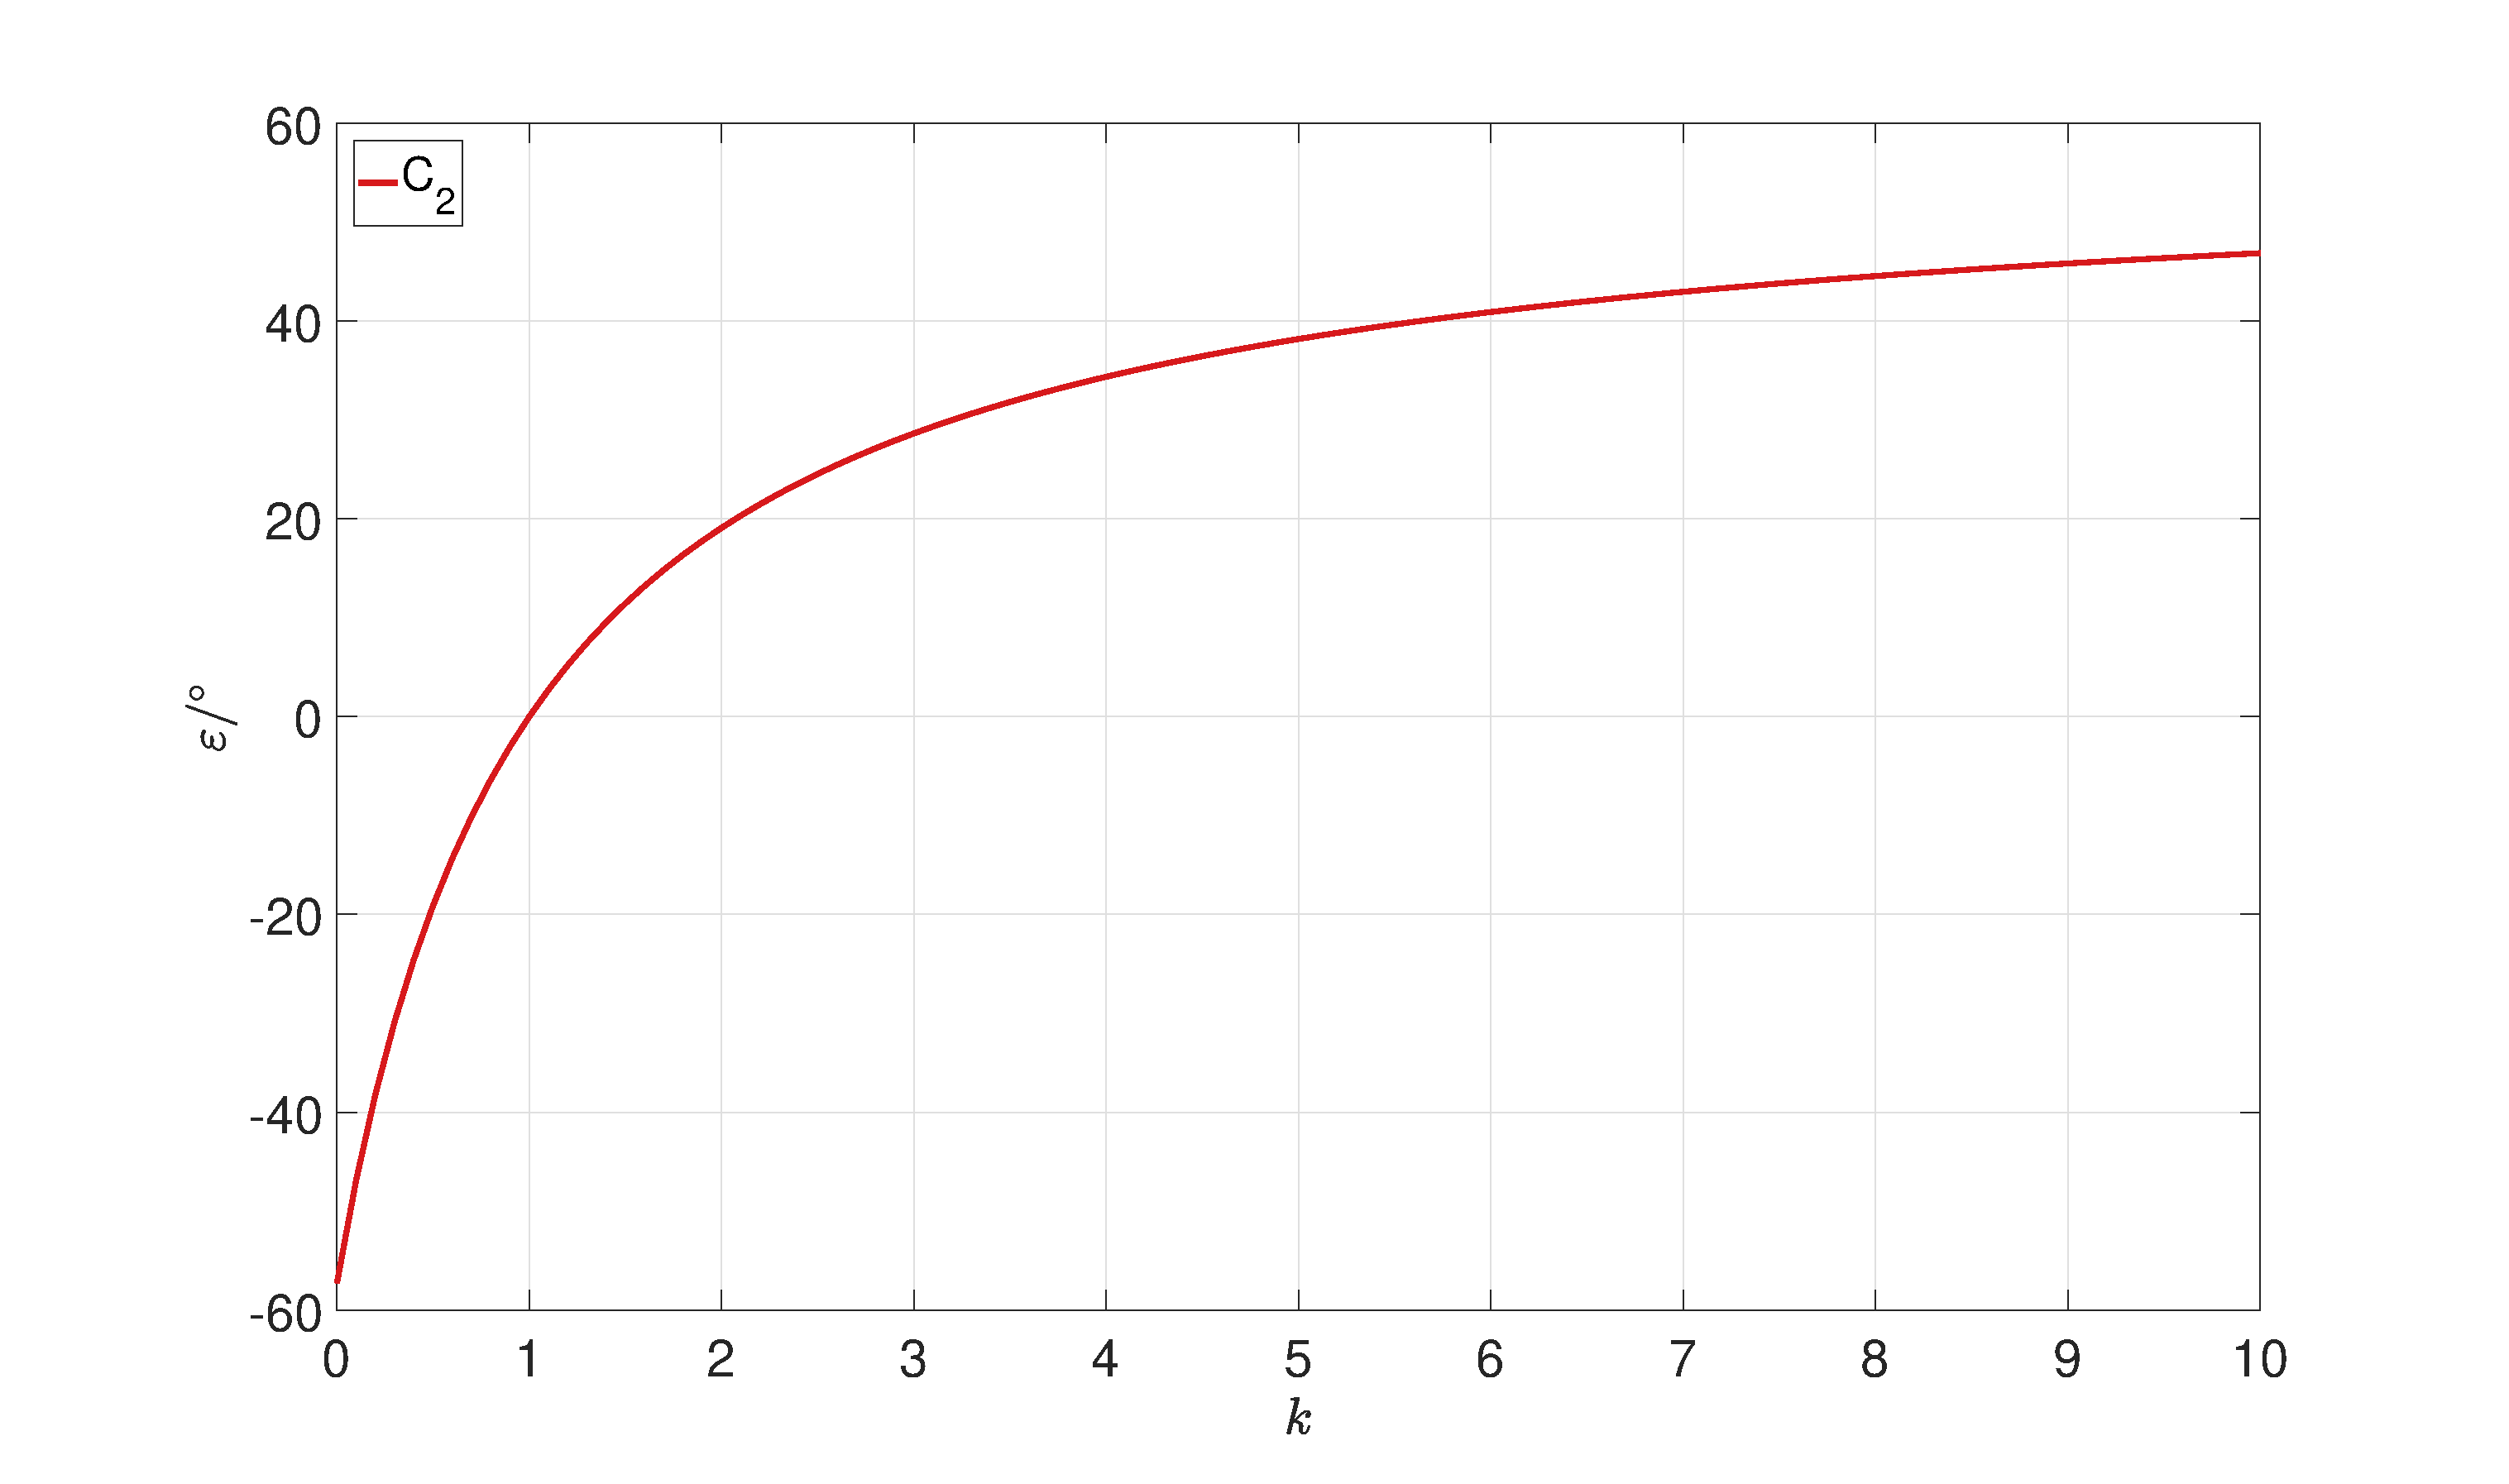
\includegraphics[width=\linewidth]{./Slike/amp.eps}
		\caption{Potek drugega harmonika v odvistnosti od k} \label{fig:amp}
	\end{center}
\end{figure}
Z uporabo Curve Fitting Toolbox se najbolje prilega poteku  racionalna funkcija.

\begin{equation}
\label{equ:amp_err}
\varepsilon(k) =\frac{180}{\pi}\sum_{n=1}^{\infty}\frac{1}{n}(\frac{k-1}{k+1})^n \sin 2 n \theta
\end{equation}

Izraz velja, če je k večji od 0.$$k \geq 0$$

\subsection{Določanje napake ob spremembi parametra $\varphi_{s}$}


Vhodna signala imata naslednjo obliko:
\begin{eqnarray}
\label{equ:def_sin_fis}
&Sin = \sin(\theta + \varphi_{s})\\
\label{equ:def_cos_fis}
&Cos =\cos(\theta)
\end{eqnarray}
Za določanje limite, v tem primeru, ni potrebno iti proti neskončnosti, ampak le do najslabše možnosti, ki je pri $90^\circ$ oz $-90^\circ$:
\begin{equation}
\label{equ:fis_lim}
\varepsilon = \lim_{\varphi_{s} \rightarrow 90^\circ} \mathrm{atan2}(Sin ,Cos)- \mathrm{atan2d}(\sin(\theta),\cos(\theta))
\end{equation}
Potek napake $\varepsilon$ s slike \ref{fig:lim_sin_fis} predstavi vrsta (\ref{equ:lim_fis_vrsta}).
\begin{figure}[!htb]
    \begin{center}
        \includegraphics[width=\linewidth]{./Slike/lim_sinfaza.eps}
        \caption{Napaka $\varepsilon$ ob limiti $\varphi_{s} = 90^\circ$} \label{fig:lim_sin_fis}
    \end{center}
\end{figure}
\begin{equation}
\label{equ:lim_fis_vrsta}
\varepsilon = 45^\circ - \frac{180}{\pi}\sum_{n=1}^{\infty}\frac{1}{n} \sin (2n \theta)
\end{equation} 
Iz  izraza je vidno, nastopanje enosmerne komponente in sodih harmonikov. Na sliki \ref{fig:fis} so prikazani: potek enosmerne komponente $C_0$, potek amplitude drugega harmonika $C_1$, in $\varphi_1$ kot fazni zamik drugega harmonika glede na kosinusno obliko.Za predstavitev poteka s sinusi, je potrebno prišteti še $90^\circ$. Ordinatna skala grafa na sliki \ref{fig:fis} je v stopinjah. Pri $C_0$ in $C_1$, stopinje predstavljajo amplitudo napake, pri $\varphi_{1}$ je na skali fazni zamik v stopinjah.
\begin{figure}[!htb]
	\begin{center}
		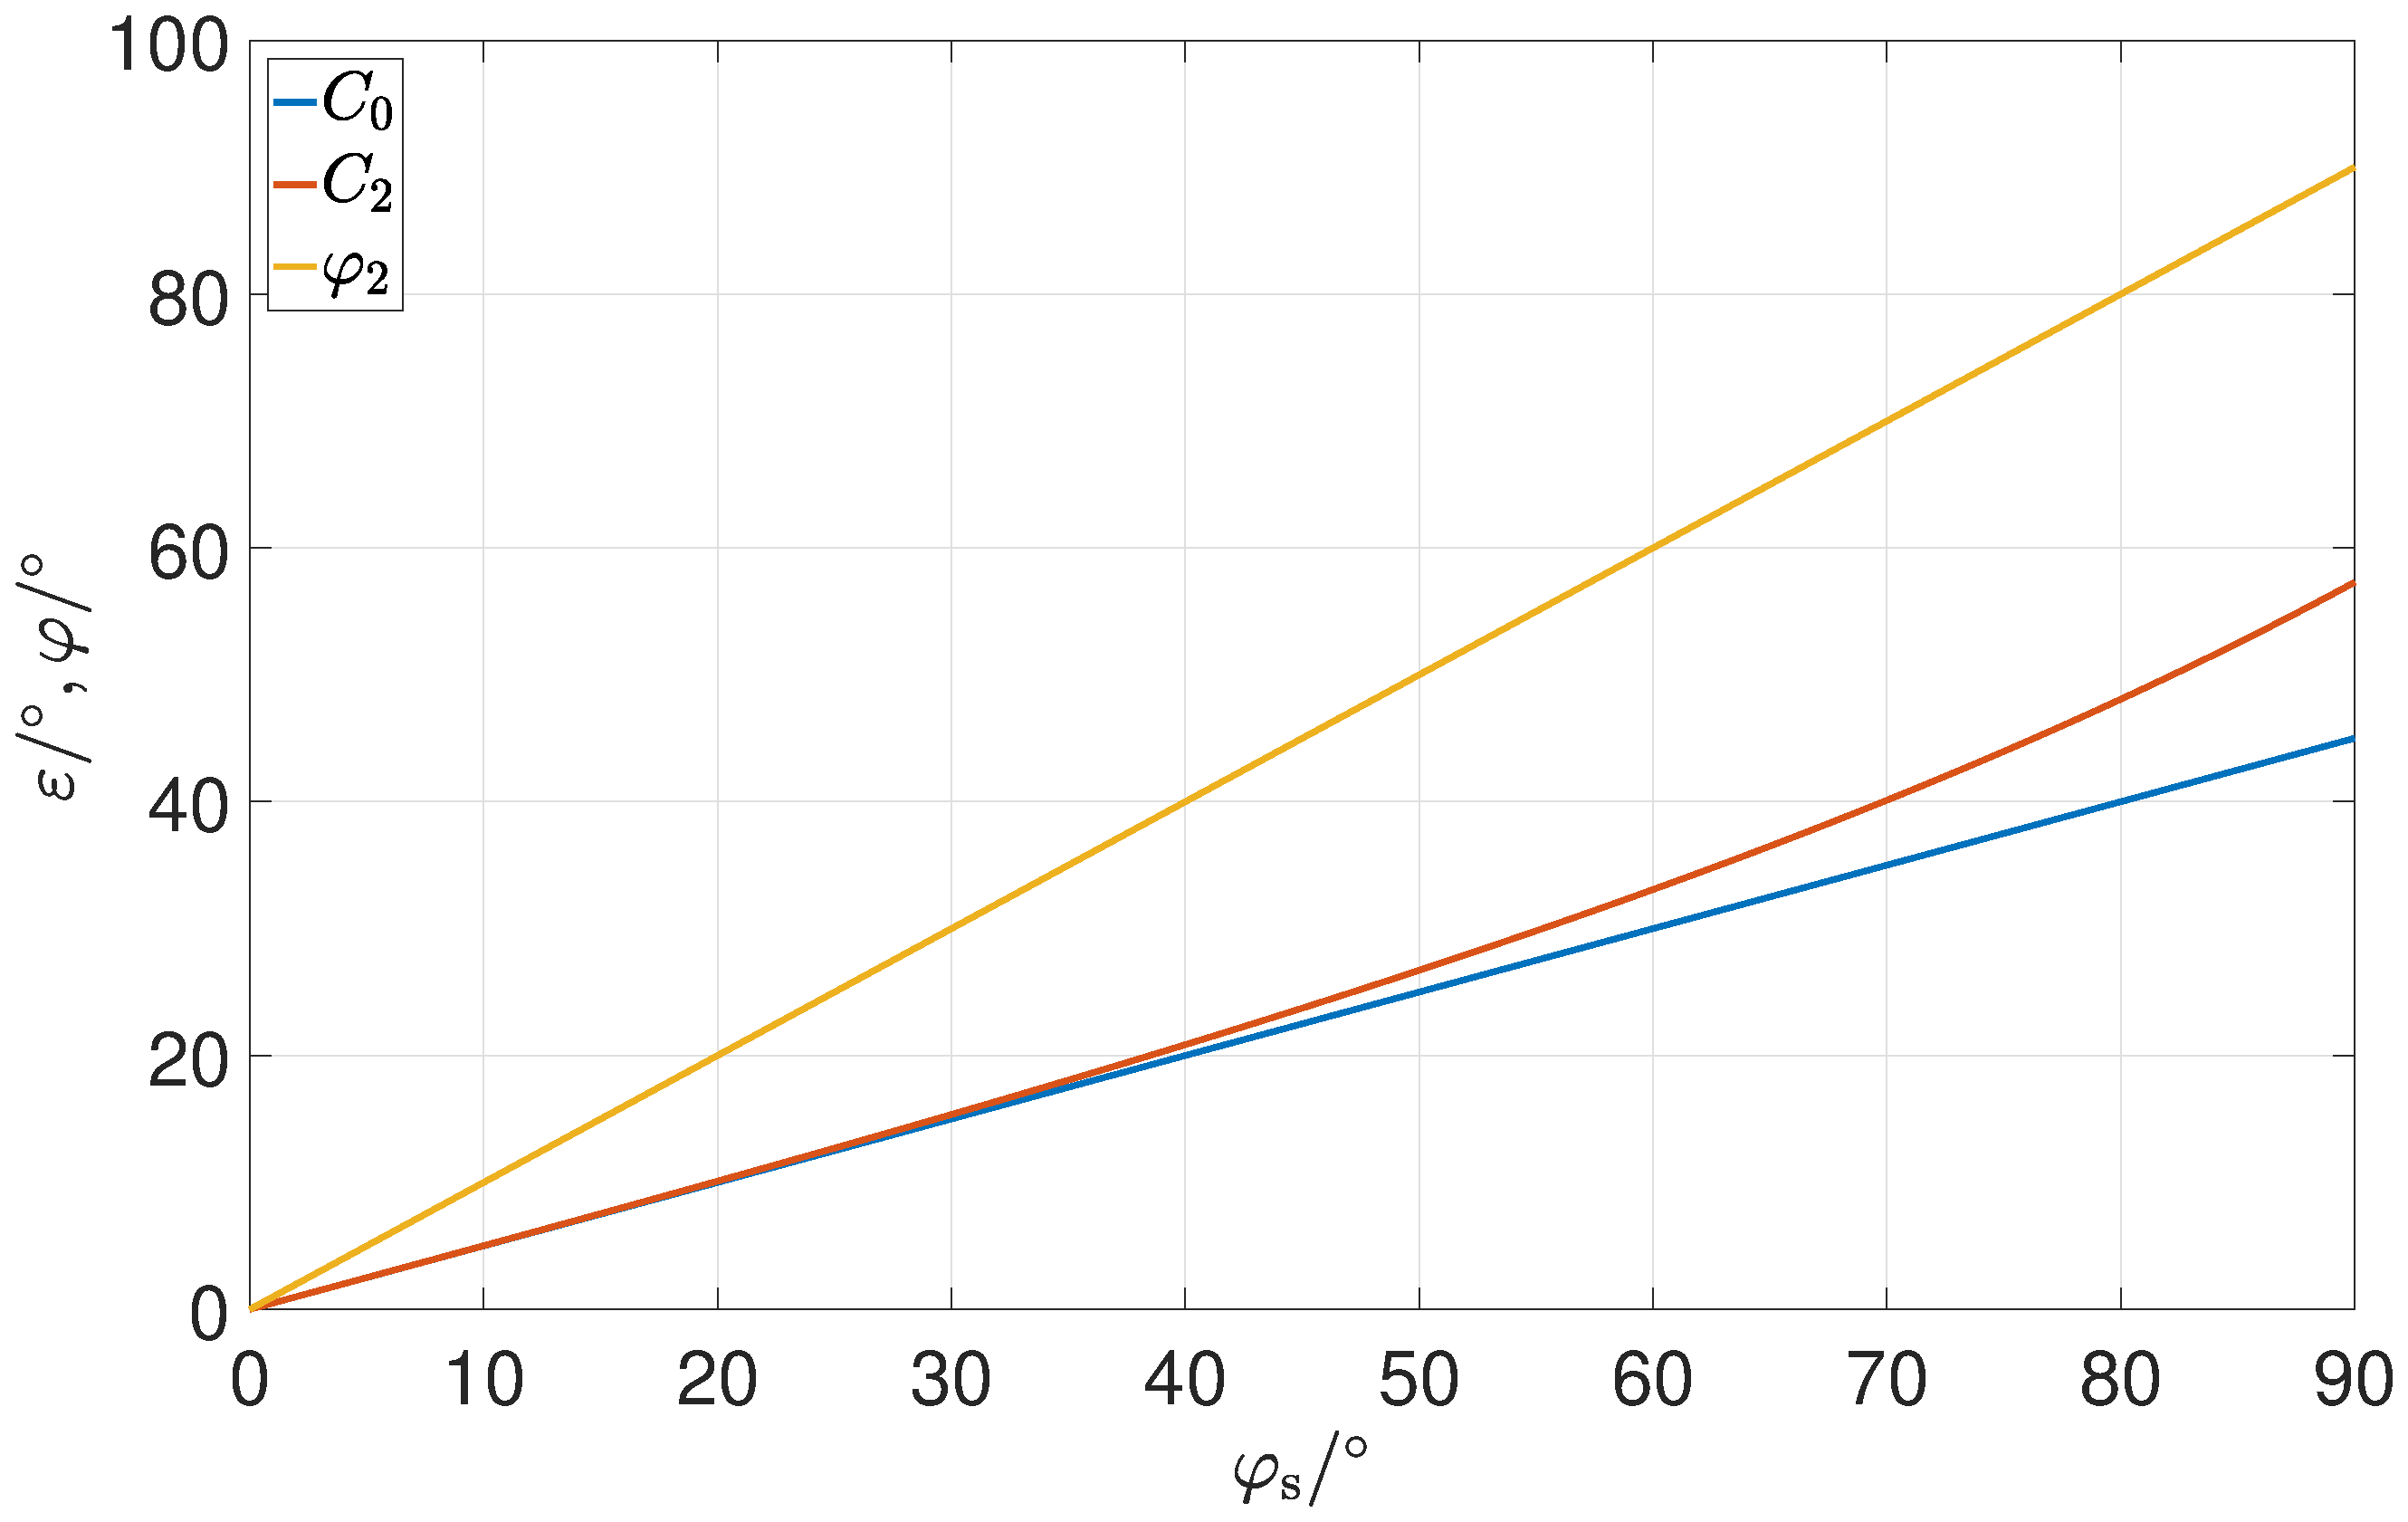
\includegraphics[width=\linewidth]{./Slike/fis.eps}
		\caption{Potek enosmerne komponente napake $C_0$, amplitude drugega harmonika $C_1$ in faznega zamika $\varphi_1$ glede na kosinus, v odvistnisti od faznega zamika sinusa $\varphi_{s}$} \label{fig:fis}
	\end{center}
\end{figure}

Potek enosmerne komponte linearen.
Potek amplitude drugega harmonika napake ima obliko funkcije tangens.

Fazni zamik drugega harmonika narašča linearno, vendar, za predstavitev s sinusi, je potrebno prišteti še $90^\circ$.

Enačba končnega poteka se glasi:
\begin{equation}
\label{equ:fis_err}
\varepsilon(\varphi_{s}) = \frac{\varphi_{s}}{2}+ \frac{180}{\pi}\sum_{n=1}^{\infty}\frac{1}{n} \mathrm{tan}(\frac{\varphi_{s}}{2})^n \sin (2n \theta+90 n +n \varphi_{sin})
\end{equation}
pri čemer velja enačba za fazne zamike sinusa med $-90^\circ$ in $90^\circ$.
$$ \varphi_{sin} \in [ -90^\circ , 90^\circ ] $$

\subsection{Določanje napake ob spremembi parametra $A_0$}

Z limito $A_0$ in razvojem napake v Fourierovo vrsto je napaka:
\begin{equation}
\label{equ:off_lim_vrsta}
\varepsilon = \frac{180}{\pi}\sum_{n=1}^{\infty}\frac{2}{n} \sin (n \theta+ 90 n)
\end{equation}
Enosmerne komponente ni,  največji je prvi harmonik.
\begin{figure}[!htb]
	\begin{center}
		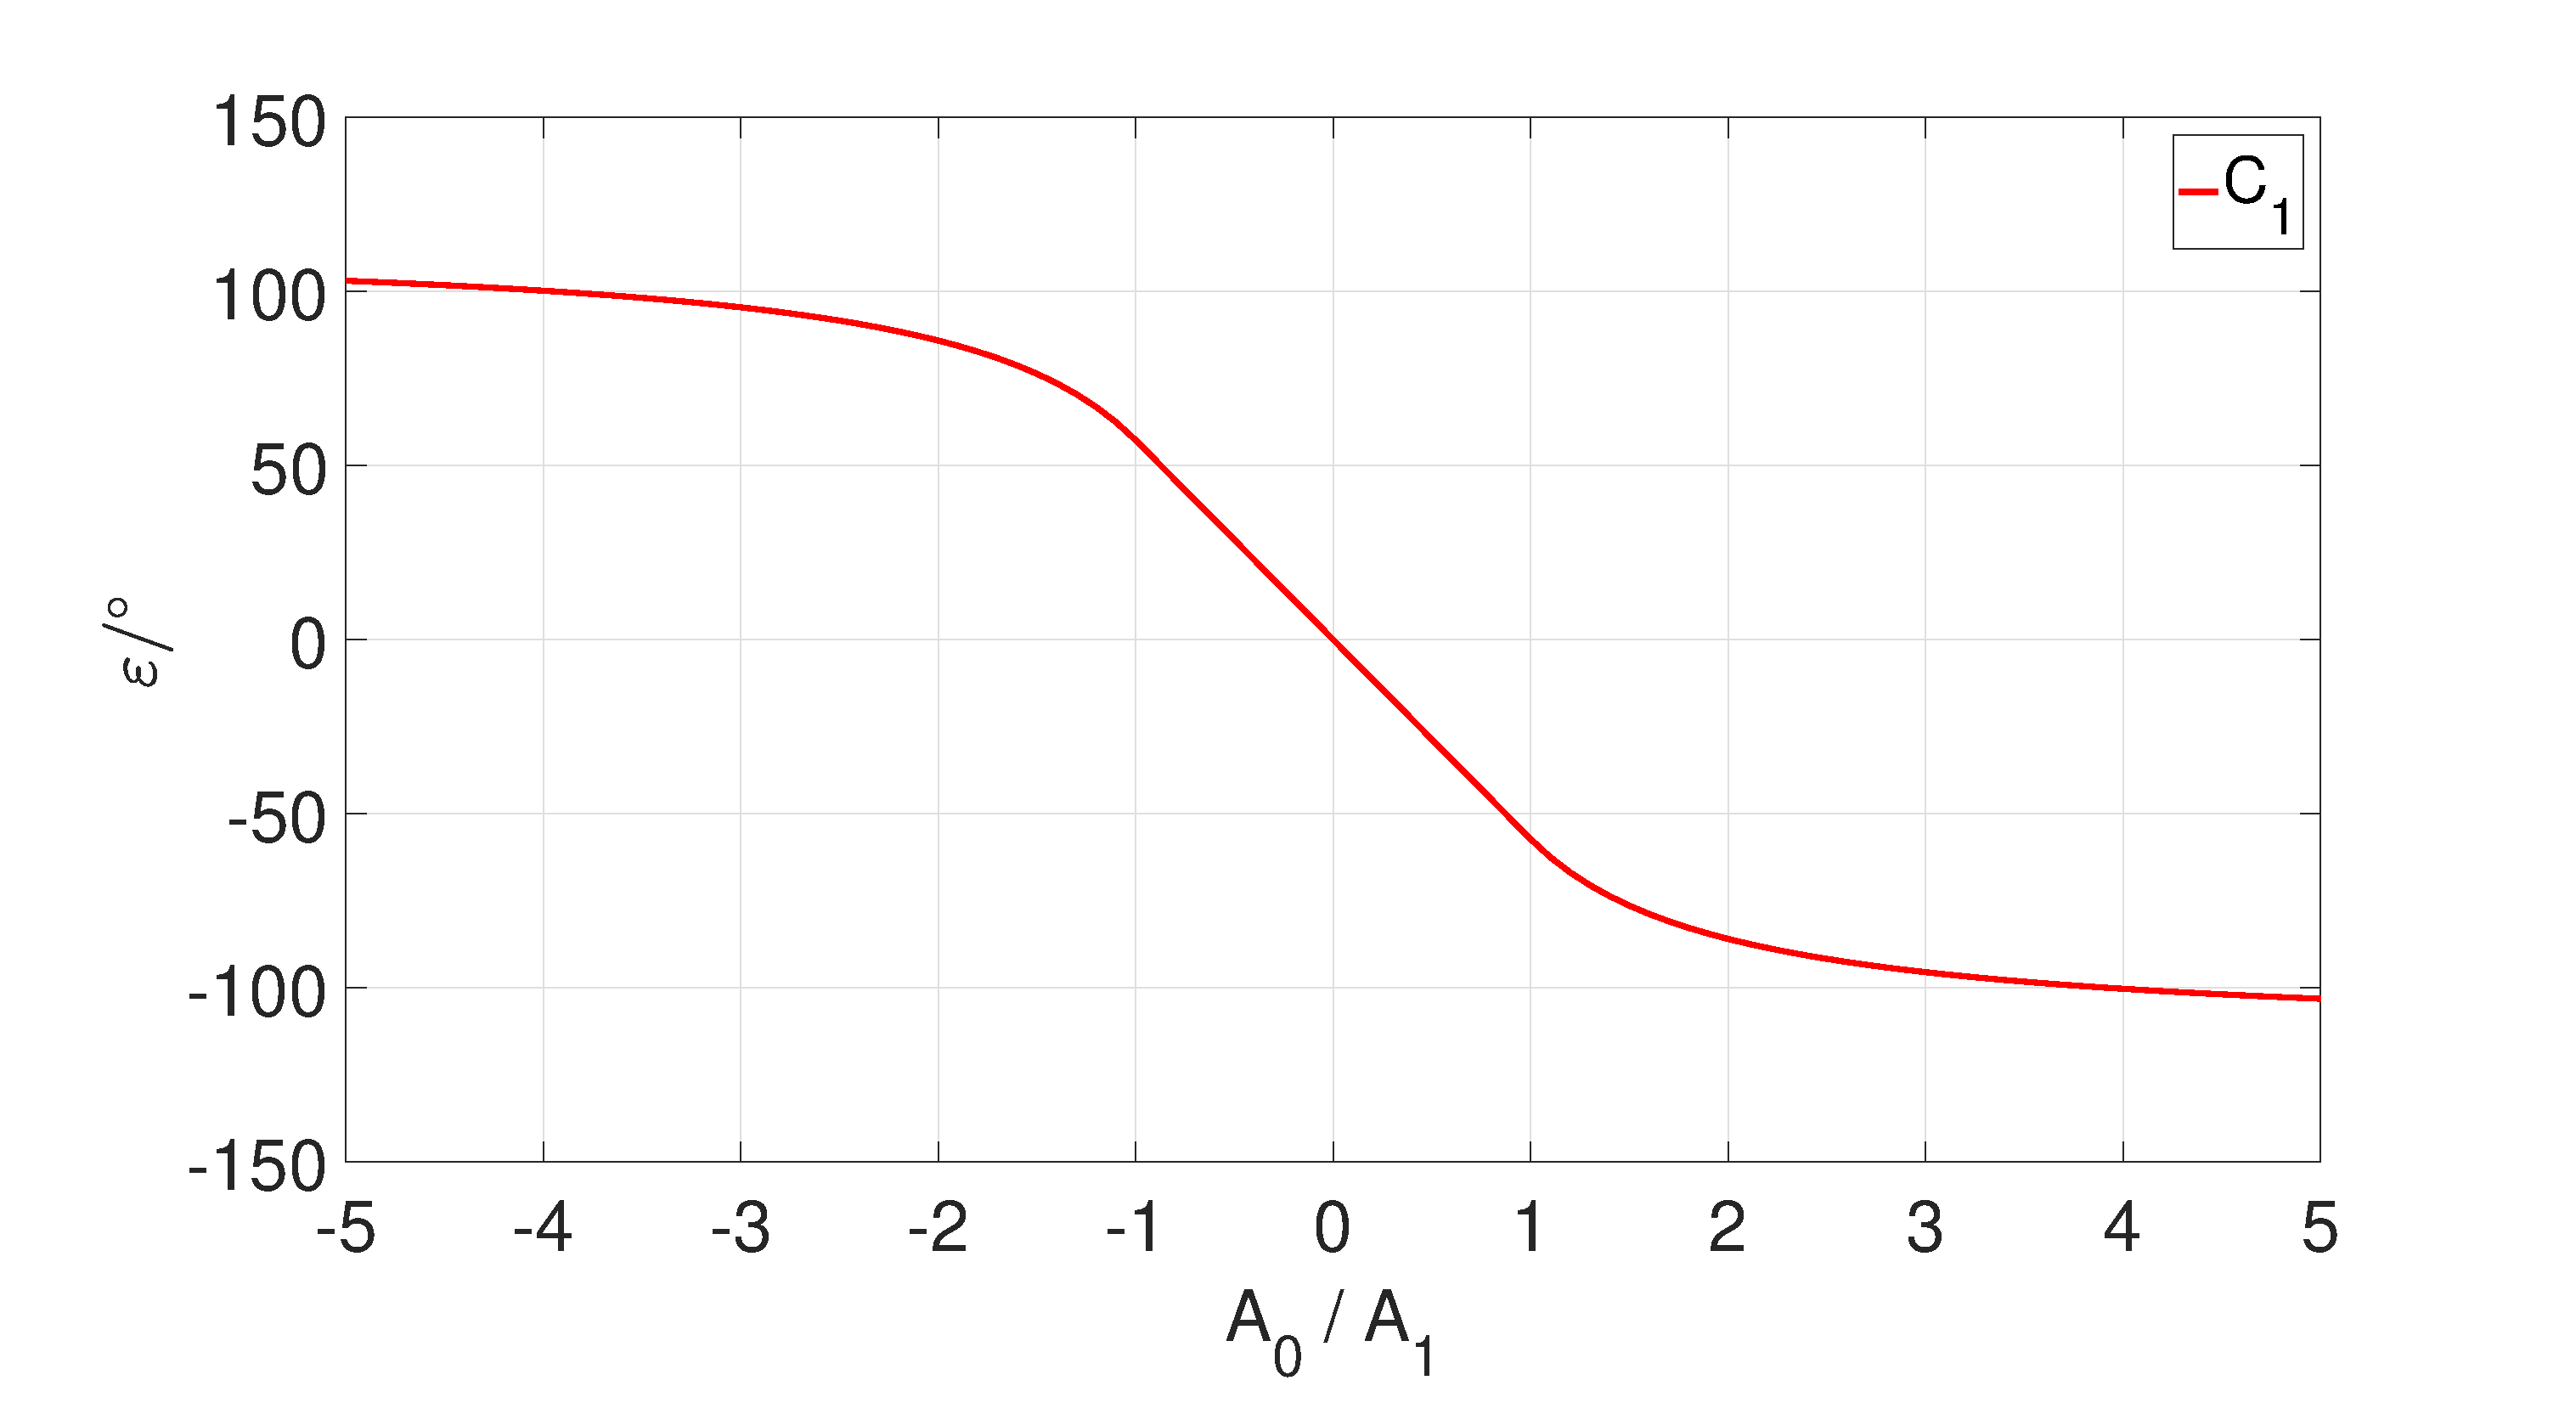
\includegraphics[width=\linewidth]{./Slike/off.eps}
		\caption{Potek amplitude prvega harmonika od enosmerne komponente kosinus signala} \label{fig:off}
	\end{center}
\end{figure}
Potek s slike \ref{fig:off} se razdeli na 3 dele in aproksimira napako z naslednjim izrazom:
\begin{equation}
\label{equ:cos_err}
\varepsilon(A_0)=
\begin{cases}
\frac{180}{\pi}\sum_{n=1}^{\infty}(-1)^n\frac{2-|A_0|^{-n}}{n} \sin (n \theta ), & A_0\leq -1 \\
\frac{180}{\pi}\sum_{n=1}^{\infty}(-1)^n\frac{A_0^n}{n} \sin (n \theta ), & |A_0|\leq 1 \\
\frac{180}{\pi}\sum_{n=1}^{\infty}(-1)^n\frac{2-A_0^{-n}}{n} \sin (n \theta ), & A_0\geq 1
\end{cases}
\end{equation}

\subsection{Dodan signal $\Delta_c \cos(\theta)$}
Fourierova vrsta limite, ko gre $\Delta_c \cos(\theta)$ v neskončnost je
\begin{equation}
\label{equ:lim_dc_vrsta}
\varepsilon = 45^\circ -\frac{180}{\pi}\sum_{n=1}^{\infty}\frac{1}{n} \sin( 2 n \theta)
\end{equation}

Drugi harmonik je predstavljen kot vsota sinusa in cosinusa.
\begin{equation}
C_1s \cdot\sin(2\theta)+C_1c \cdot\cos(2\theta)
\end{equation}
Poteki enosmerne komponente ter drugega harmonika predstavljenega kot seštevek sinusa in kosinusa so prikazani na sliki \ref{fig:dc}.
\begin{figure}[!htb]
	\begin{center}
		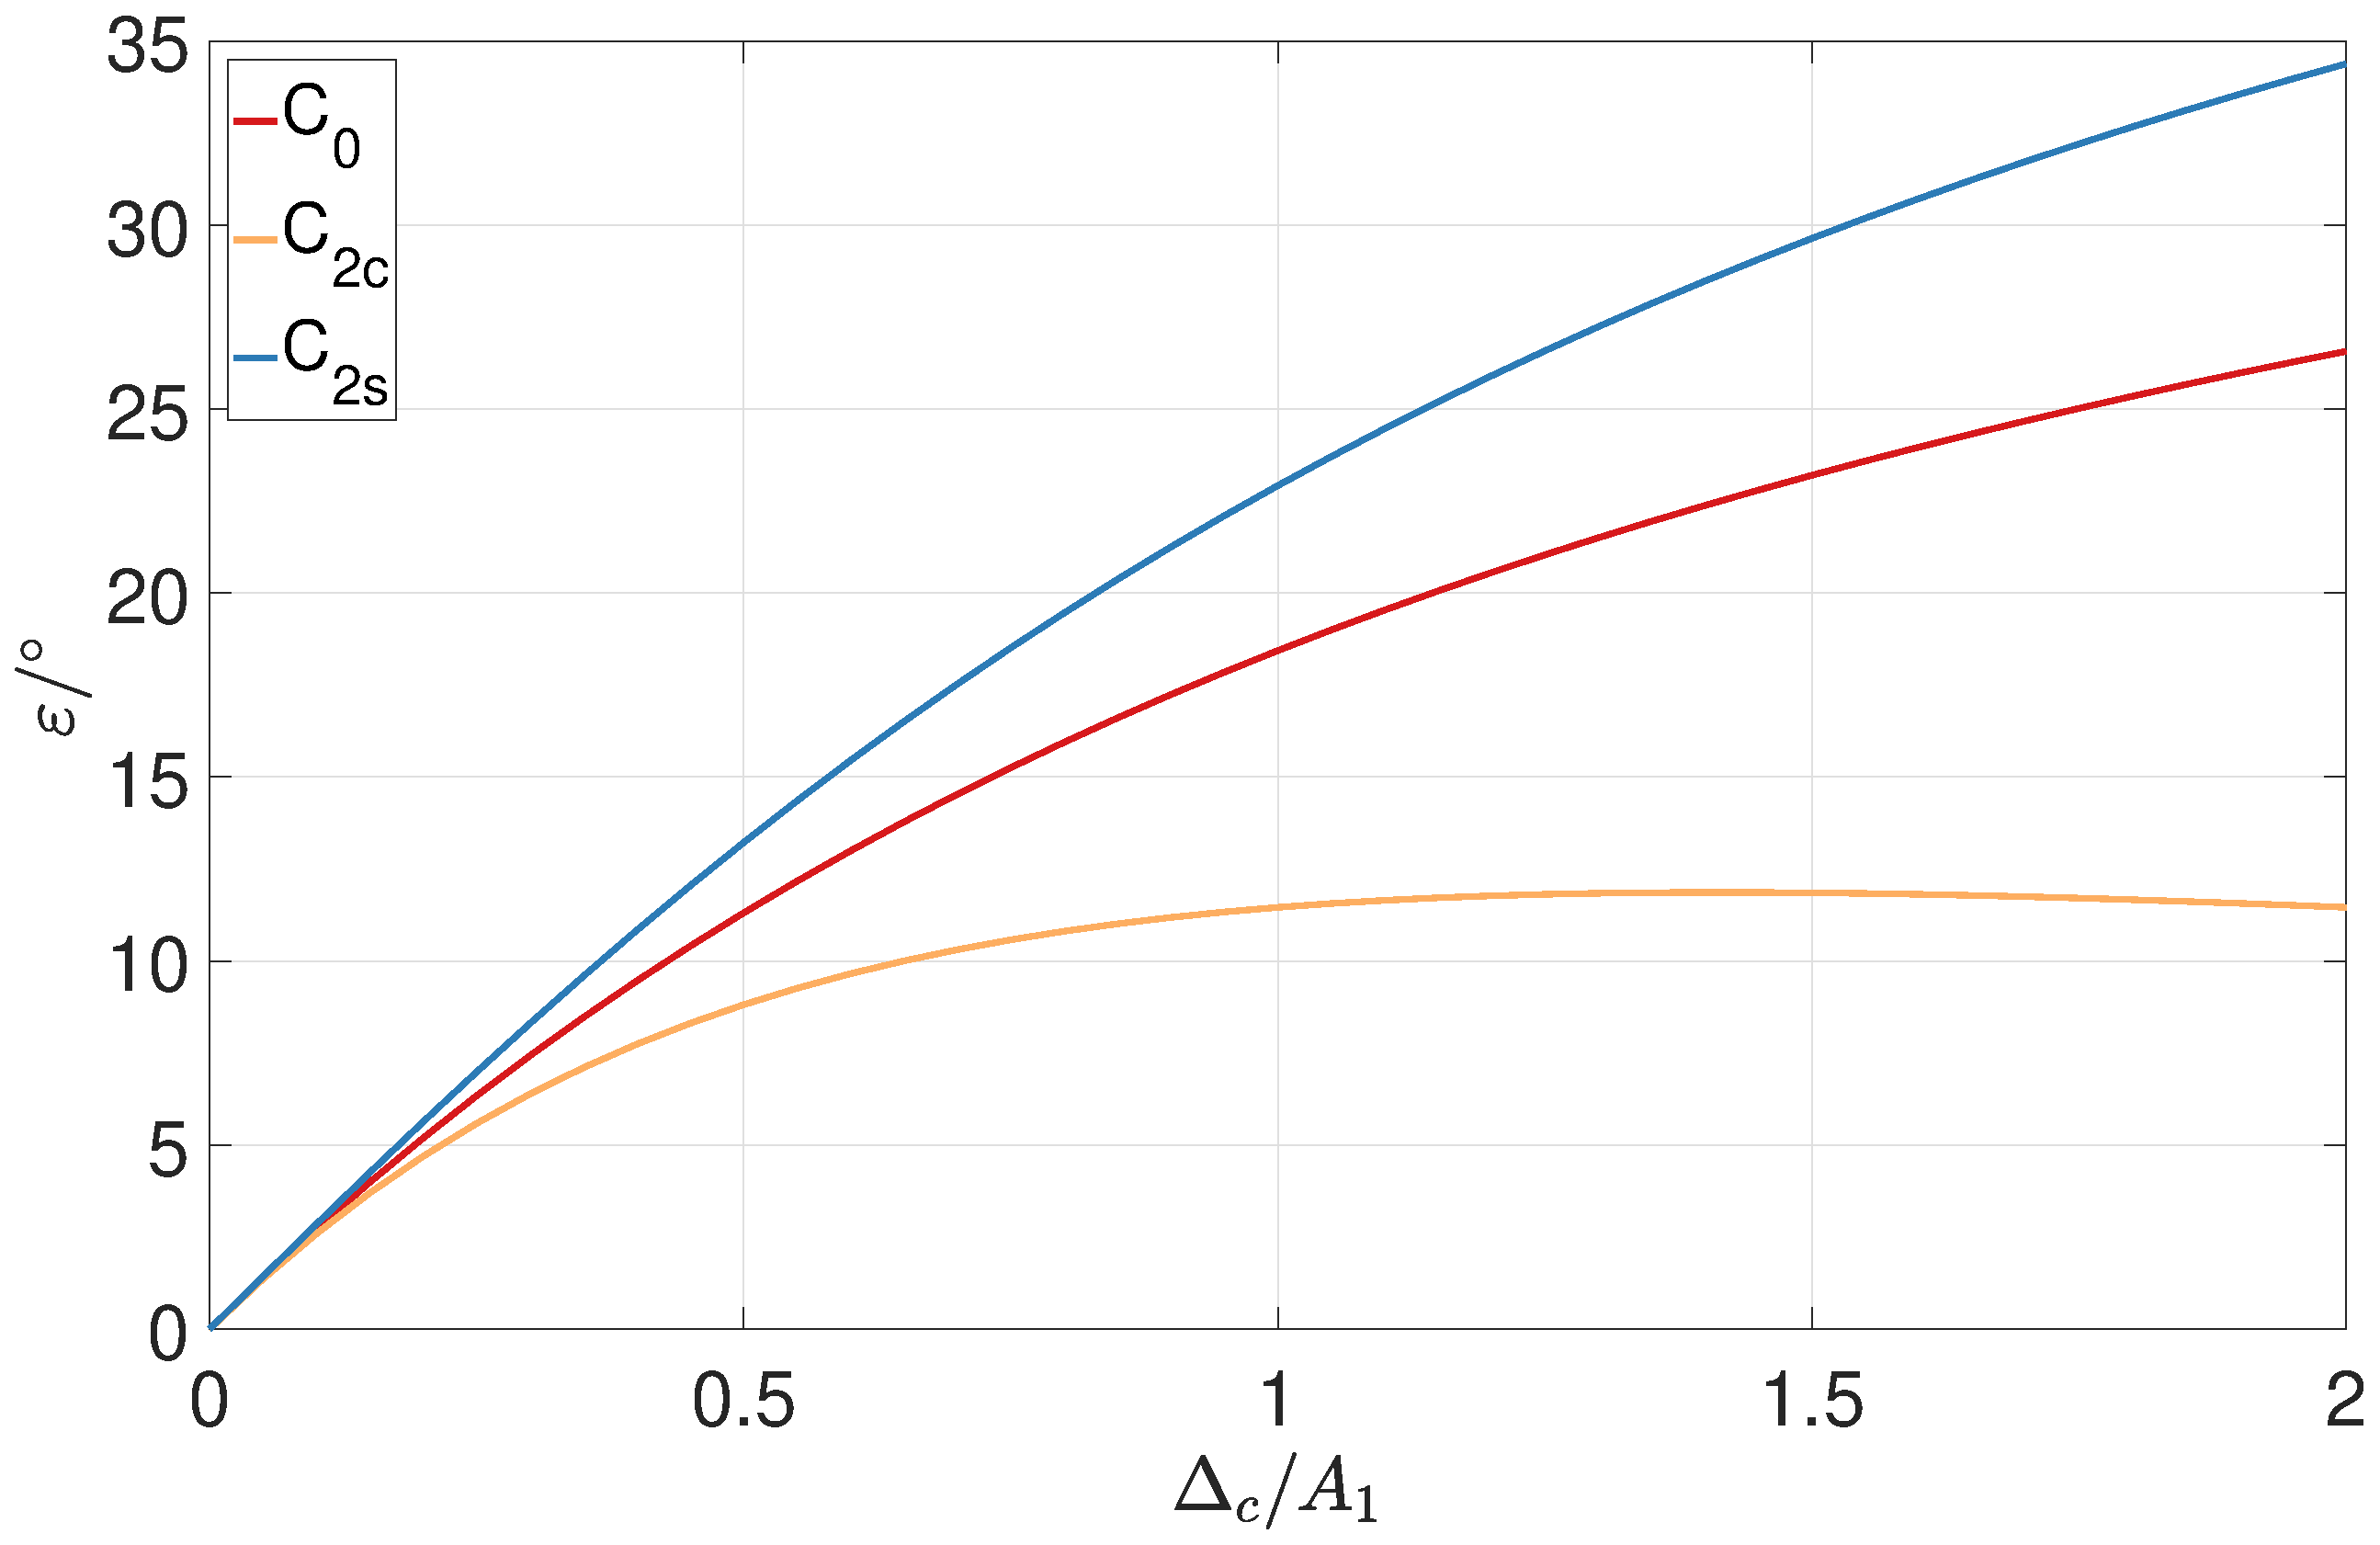
\includegraphics[width=\linewidth]{./Slike/dc.eps}
		\caption{Potek enosmerne komponente napake, v odvistnisti od faznega zamika sinusa $\varphi_{s}$} \label{fig:dc}
	\end{center}
\end{figure}

Enosmerno komponento ima obliko racionalne funkcije v funkciji atan.
$C_1s$ in $C_1c$ sti racionlni funkciji. S poznavanja funkcij, se določi skupna amplituda $C_1 = \sqrt{C_1s^2+C_1c^2}$ in faza za sinusni potek napake $\varphi_{1} = atan(\frac{C_1c}{C_1s})$. Končna enačba se glasi:

 \begin{multline}
\label{equ:dc_err}
\varepsilon(\Delta_c) = \mathrm{atand}\frac{\Delta_c}{\Delta_c+2}+\frac{180}{\pi} \sum_{n=1}^{\infty}\frac{1}{n} (\frac{\Delta_c}{\sqrt{\Delta_c^2+2 \Delta_c+2}})^n \\ \sin (2n \theta+n (90+ \mathrm{ atan}(\Delta_c+1)))
\end{multline}

Pri čemer velja, da mora biti $\Delta_c > -1$.


\section{Rezultati}

Pri modeliranju potekov, sem uporabil prvih 15 členov. Razlika med dejansko napako in predvideno napako je bila le numerična (Slika \ref{fig:razlika}). V primeru, da parameter dosega večje vrednosti, dejanska napaka postane nezvezna, je s 15 členi ni mogoče povsem zadeti, saj so odstopanja na nezveznih območjih. Omenti je še potrebno, da so kljub izpeljavam vrste s katerimi so predstavljene napake posameznih deformacij med seboj odvisne. To področje je potrebno še raziskati. Zanimivo je tudi, kako višji harmoniki vplivajo na napako.

\begin{figure}[!htb]
	\begin{center}
		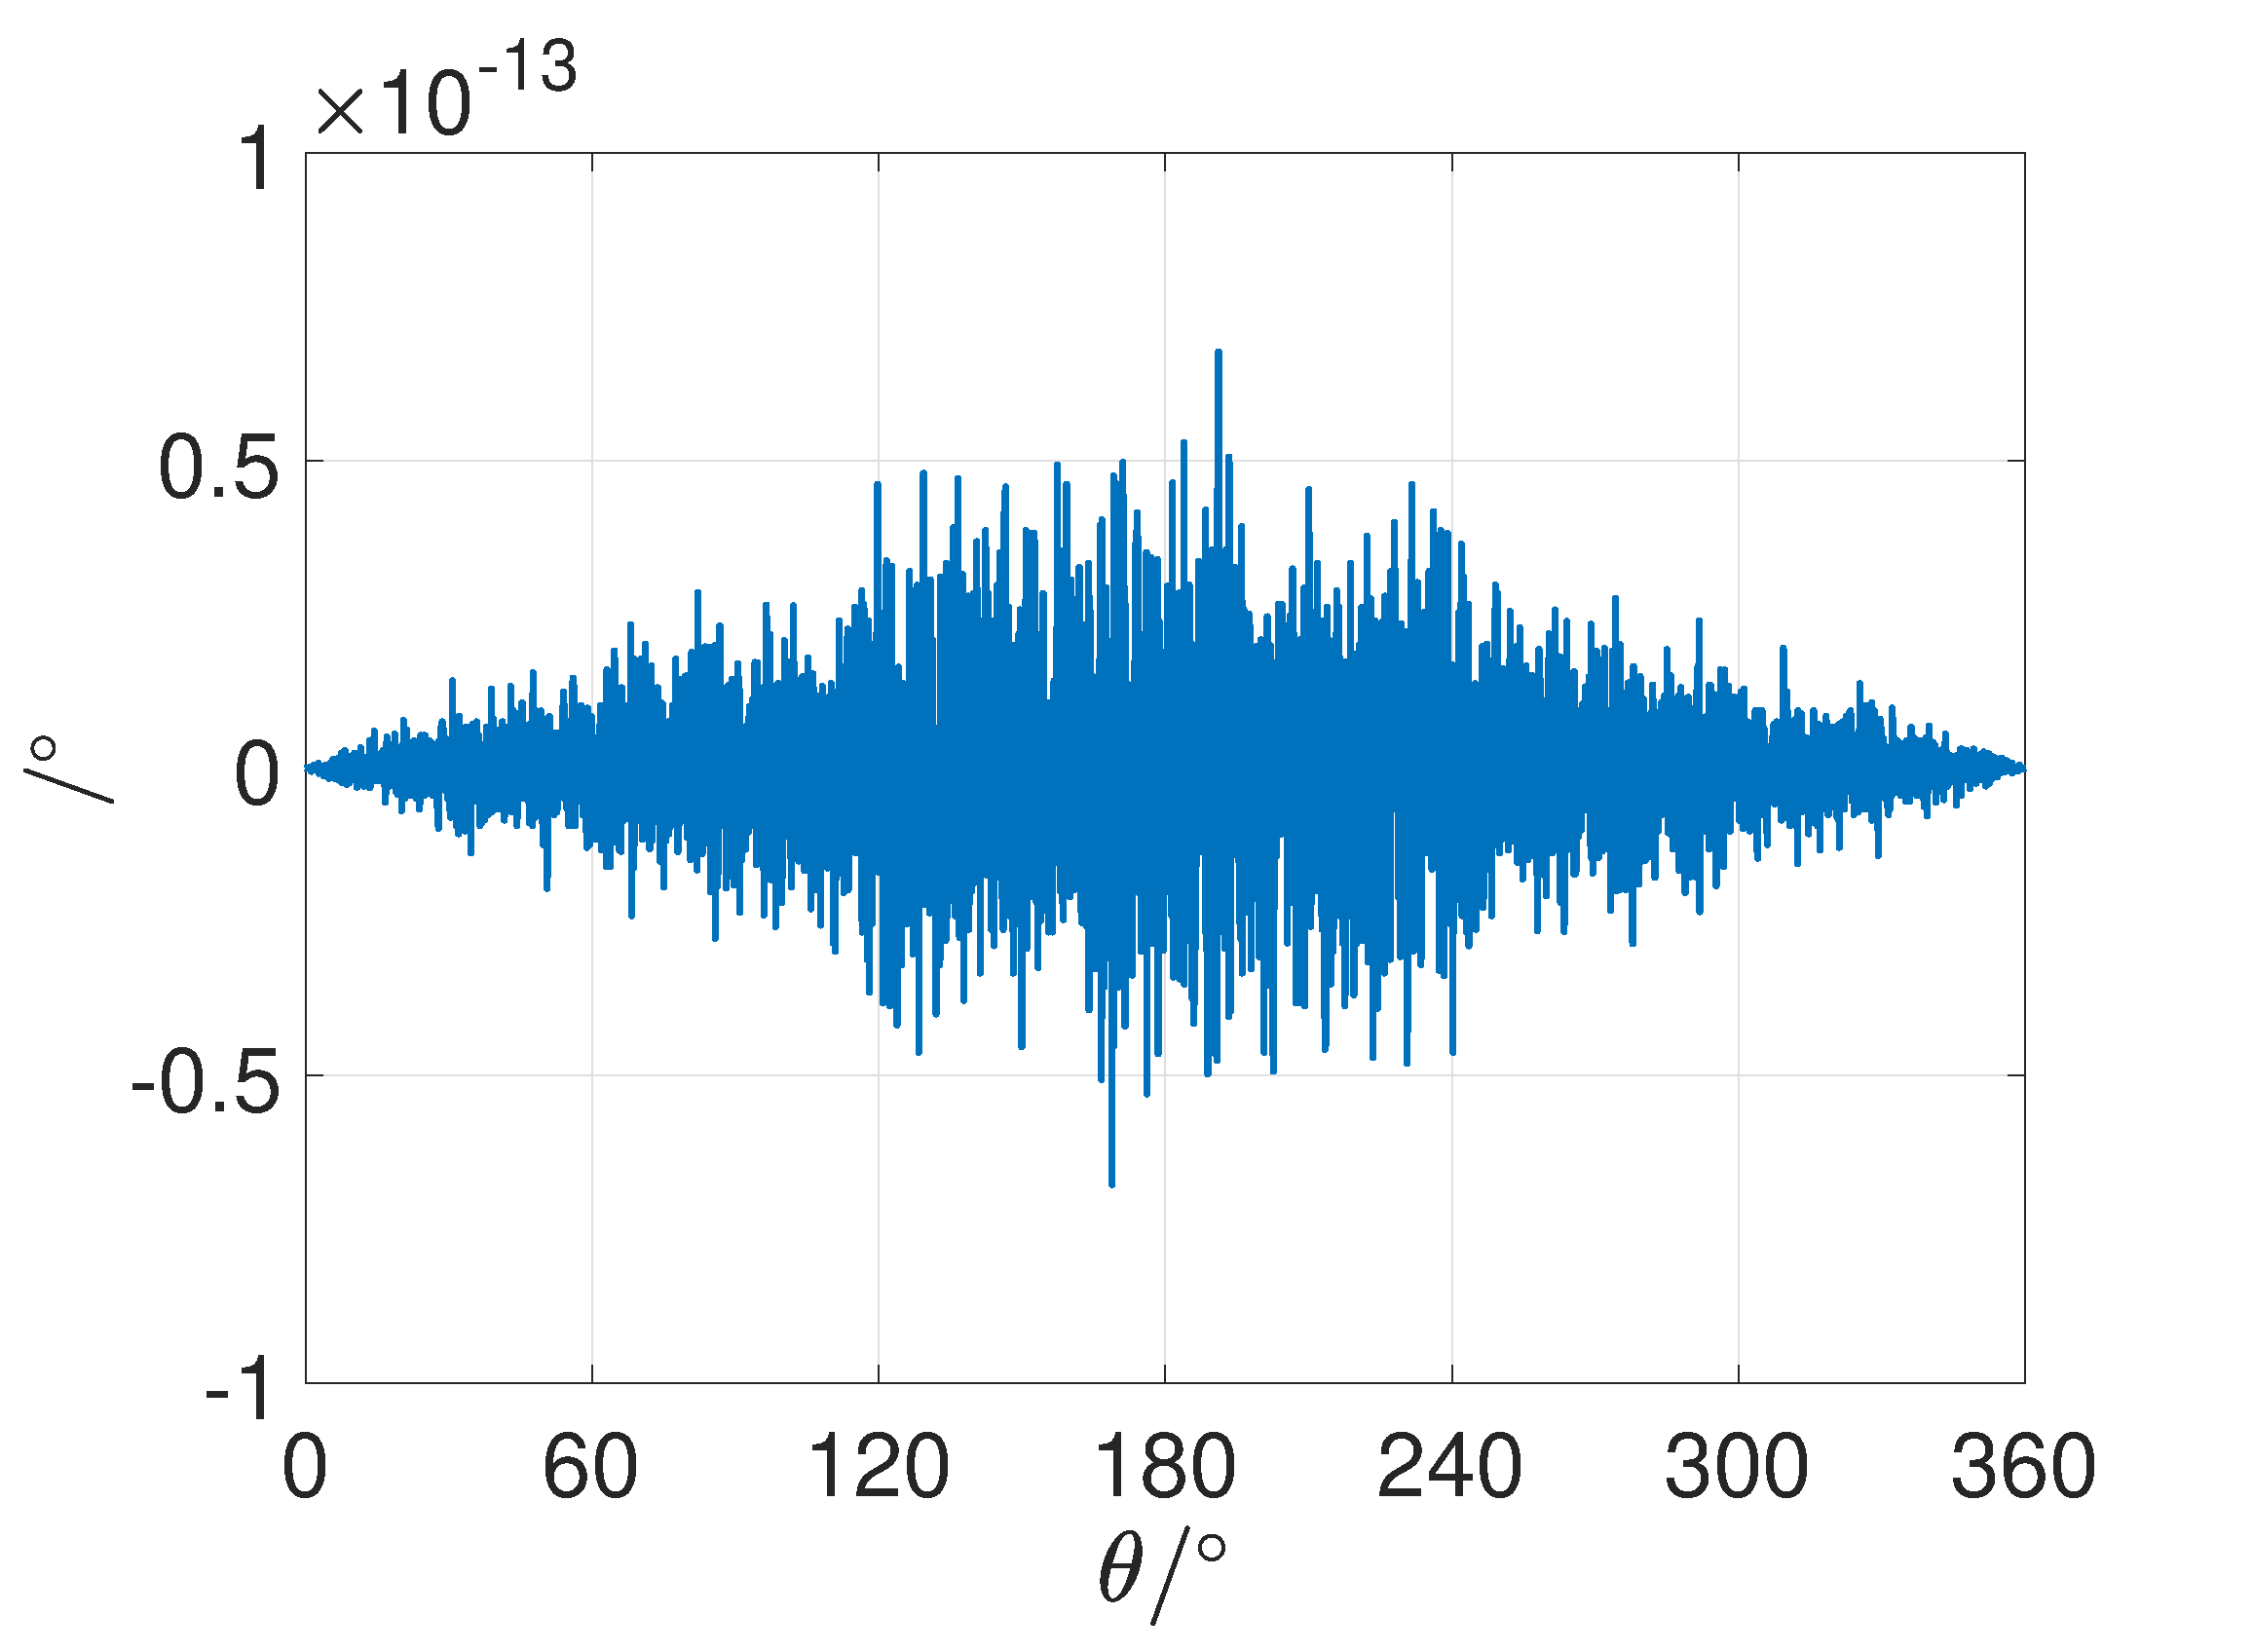
\includegraphics[width=\linewidth]{./Slike/razlika_amp.eps}
		\caption{Razlika med predvidvideno napako (\ref{equ:amp_err}) in dejansko numerično izračunano napako pri $k=1.1$} \label{fig:razlika}
	\end{center}
\end{figure}


Sedaj izpišem še vse rezultate:

\begin{equation}
\varepsilon(k) =\frac{180}{\pi}\sum_{n=1}^{\infty}\frac{1}{n}(\frac{k-1}{k+1})^n \sin 2 n \theta
\end{equation}
\begin{equation*}
k \geq 0
\end{equation*}
\begin{equation*}
k = \frac{B_1}{A_1}
\end{equation*}
\begin{equation}
\varepsilon(\varphi_{s}) = \frac{\varphi_{s}}{2}+ \frac{180}{\pi}\sum_{n=1}^{\infty}\frac{1}{n} \mathrm{tan}(\frac{\varphi_{s}}{2})^n \sin (2n \theta+90 n +n \varphi_{s})\\
\end{equation}
\begin{equation*}
\varphi_{s} \in [-90^\circ, 90^\circ]
\end{equation*}
\begin{equation}
\varepsilon(\varphi_{c}) = \frac{\varphi_{c}}{2}+ \frac{180}{\pi}\sum_{n=1}^{\infty}\frac{1}{n} \mathrm{tan}(\frac{\varphi_{c}}{2})^n \sin (2n \theta-90 n +n \varphi_{c})\\
\end{equation}
\begin{equation*}
\varphi_{c} \in [-90^\circ, 90^\circ]
\end{equation*}
\begin{multline}
\varepsilon(B_0)=\\
\begin{cases}
\frac{180}{\pi}\sum_{n=1}^{\infty}\frac{2-|B_0|^{-n}}{n} \sin (n \theta -  90 n), & B_0\leq -1 \\
\frac{180}{\pi}\sum_{n=1}^{\infty}\frac{B_0^n}{n} \sin (n \theta + 90 n), & |B_0|\leq 1 \\
\frac{180}{\pi}\sum_{n=1}^{\infty}\frac{2-B_0^{-n}}{n} \sin (n \theta + 90 n), & B_0\geq 1
\end{cases}
\end{multline}
\begin{multline}
\varepsilon(A_0)=\\
\begin{cases}
\frac{180}{\pi}\sum_{n=1}^{\infty}(-1)^n\frac{2-|A_0|^{-n}}{n} \sin (n \theta ), & A_0\leq -1 \\
\frac{180}{\pi}\sum_{n=1}^{\infty}(-1)^n\frac{A_0^n}{n} \sin (n \theta ), & |A_0|\leq 1 \\
\frac{180}{\pi}\sum_{n=1}^{\infty}(-1)^n\frac{2-A_0^{-n}}{n} \sin (n \theta ), & A_0\geq 1
\end{cases}
\end{multline}
\begin{multline}
\varepsilon(A_0,B_0=A_0)=\\
\begin{cases}
\frac{180}{\pi}\sum_{n=1}^{\infty}\frac{2-|\sqrt{2}A_0|^{-n}}{n} \sin (n \theta + 90 n), & A_0\leq -\frac{\sqrt{2}}{2} \\
\frac{180}{\pi}\sum_{n=1}^{\infty}\frac{(\sqrt{2}A_0)^n}{n} \sin (n \theta - 90 n), & |A_0|\leq \frac{\sqrt{2}}{2} \\
\frac{180}{\pi}\sum_{n=1}^{\infty}\frac{2-(\sqrt{2}A_0)^{-n}}{n} \sin (n \theta - 90 n), & A_0\geq \frac{\sqrt{2}}{2}
\end{cases}
\end{multline}
\begin{multline}
\varepsilon(\Delta_c) = \mathrm{atand}\frac{\Delta_c}{\Delta_c+2}+\frac{180}{\pi} \sum_{n=1}^{\infty}\frac{1}{n} (\frac{\Delta_c}{\sqrt{\Delta_c^2+2 \Delta_c+2}})^n\\ \sin (2n \theta+n (90+ \mathrm{ atan}(\Delta_c+1)))
\end{multline}
\begin{equation*}
\Delta_c > -1
\end{equation*}
\begin{multline}
\varepsilon(\Delta_s) = \mathrm{atand}\frac{-\Delta_s}{\Delta_s+2}+\frac{180}{\pi} \sum_{n=1}^{\infty}\frac{1}{n} (\frac{\Delta_s}{\sqrt{\Delta_s^2+2 \Delta_s+2}})^n\\ \sin (2n \theta+n (90+ \mathrm{ atan}(\Delta_s+1)))
\end{multline}
\begin{equation*}
\Delta_s > -1
\end{equation*}

\section{Zaključek}

Spoznali smo kako se napaka razvija glede na deformacijo sinusnega in kosinusnega signala. Prikazal sem, kam bo napaka limitirala in katere harmonike je potrebno opazovati. Potek harmonika napake glede na deformacijo sem želel izpeljati s najbolj prilagujočo se funkcijo, katero sem lahko odkril, a kljubtemu nezahtevno. Za majhne deformacije sinusa in kosinusa, se lahko uporabi le prvi člen vrste, kar potrjuje druga literatura. S tem delom sem želel na drugačen način prikazati obnašanje napake, ob deformaciji signalov sinus in kosinus. 

\small
\begin{thebibliography}{1}
\bibitem{RLS1} Qi Lin, Tiecai Li, Zhaoyong Zhou, "Error Analysis and Compensation
of the Orthogonal Magnetic Encoder", Proceedings of IEEE ICMCC
Conference, pp.11-14, 21-23 Oct. 2011
\bibitem{RLS2} Hanselman D.C., "Resolver Signal Requirements for High Accuracy
Resolver-to-Digital Conversion", IEEE Transactions on Industrial
Electronics, vol.37, no.6, pp.556-561, Dec. 1990 
\bibitem{RLS3} Demierre M., “Improvements of CMOS Hall Microsystems and
Application for Absolute Angular Position Measurements”, PhD. thesis,
pp. 152-161, Federal Polytechnic School of Lausanne, Switzerland, 2003 
\bibitem{atan} https://www.mathworks.com/help/matlab/ref/atan2d.html
\bibitem{fourier} https://sl.wikipedia.org/wiki/Fourierova\_vrsta


\end{thebibliography}

\end{document}
